%Elliptische Kurven


\chapter{Elliptische Kurven}


Als Basis für Asymentrische Kryptosysteme können elliptische Kurven dazu genutzt werden, die verschlüsselungstechnische Effektivität mathematischer Probleme, wie das des diskreten Logarithmus, zu erhöhen. Bei der Kryptographie unter Verwendung elliptsicher Kurven bei deutlich kürzerer Schlüssellänge ein gleichwertigers Ergebnis erzielt werden. Dieser Effekt wird durch die spezielle Arithmetik auf elliptischen Kurven erzielt, deren mathematische Grundlage, konkrete Eingenschaften und Funktionsweise im folgenden Kapitel erörtert werden soll.\\

Elliptische Kurven können über beliebigen Körpern definiert werden. Für die Kryptographie interessant sind elliptische Kurven über Primkörpern.

%\section{Definition: Elliptische Kurven}
% Sei \textit{p} eine \textit{Primzahl} $p>3$. Seien $a,b \in GF(p)$. Betrachte die Gleichung
%\begin{equation}
%    y^2 z = x^3 + axz^2 + bz^3.\label{eq:g1}
%\end{equation} Die \textit{Diskriminante}  dieser Gleichung ist
%\begin{equation}
%    \delta = -16(4a^3 + 27b^2).\label{eq:g2}
%\end{equation}
%Wir nehmen an, dass die Diskriminante $\delta$ nicht Null ist. Ist $(x,y,z) \in GF(p)^3$ eine Lösung dieser
%Gleichung, so ist für alle $c \in GF(p)$ auch $c(x,y,z)$ eine solche Lösung. Zwei Lösungen $(x,y,z)$ und $(x',y',z')$
%heißen \textit{äquivalent}, wenn es ein von Null verchiedenes $c \in GF(p)$ gibt mit $(x,y,z) = c(x',y',z')$. Dies
%definiert eine Äquivalenzrelation auf der Menge aller Lösungen der~\eqref{eq:g1}.




Um das weitere Verständnis zu verbessern, wollen wir erst eine uns schon bekannte Kurve ansehen. In Abbildung XY ist das Polynom $x^2 + y^2 = r^2$ über $\mathbb{R}$ dargestellt. Wie zu sehen ist, handelt es sich hierbei um die Kreisgleichung. Der zu sehende Kreis ist nichts anderes als die Menge aller Punkte, welche die Kreisgleichung erfüllen.
Ein Beispiel für eine solchen ist der Punkt $(r,0)$. Wenn $x$ den Wert $r$ hat, muss $y$ folglich den Wert $0$ haben. Ein Gegenbeispiel ist der Punkt $(r,r/2)$. Dieser erfüllt die Kreisgleichung nicht.
\begin{figure}[!h]
    \centering
    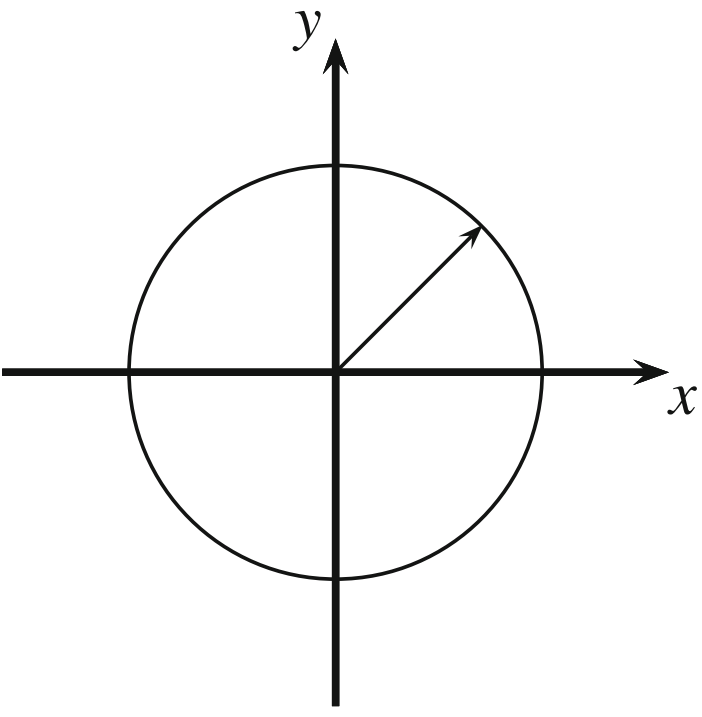
\includegraphics[width=0.3\textwidth]{grafiken/Kreis.PNG}
    \caption[r]{r}
    \label{fig:aufgaben_redesign}
\end{figure}
Die Kreisgleichung kann verallgemeinert werden, indem den Termen $x^2$ und $y^2$ Koeffizienten voran gesetzt werden. Eine solche Gleichung, $ax^2 + by^2 = c$ erzeugt über $\mathbb{R}$ eine Ellipse, wie in Abbildung XY zu sehen.
\begin{figure}[H]
    \centering
    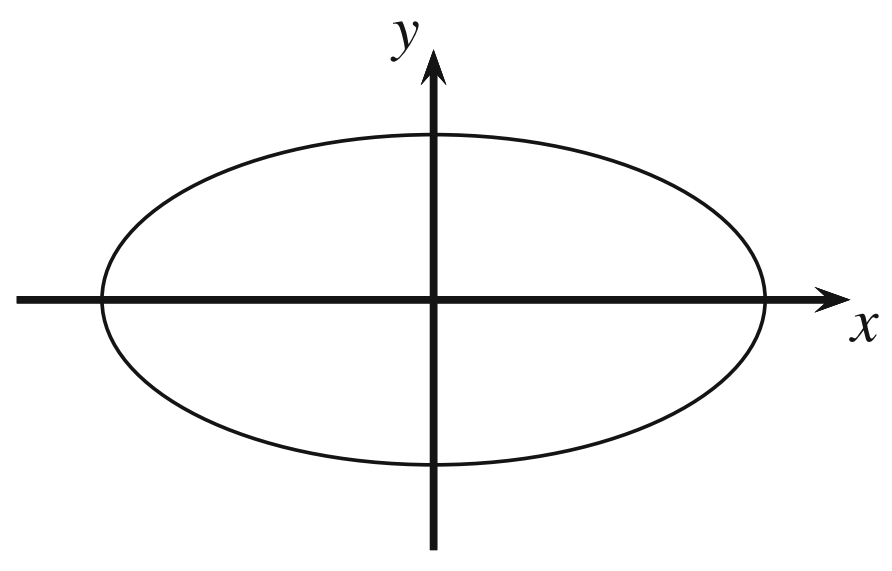
\includegraphics[width=0.3\textwidth]{grafiken/Ellipse.PNG}
    \caption[r]{r}
    \label{fig:aufgaben_redesign}
\end{figure}
Eine elliptische Kurve ist nun eine spezielle Polynomgleichung, der Form $y^2 = x^3 + ax + b$, unter der Bedingung $4a^3 + 27b^3 \neq 0$. Eine solche Gleichung über $\mathbb{R}$ ist in Abbildung XY dargestellt.
\begin{figure}[!h]
    \centering
    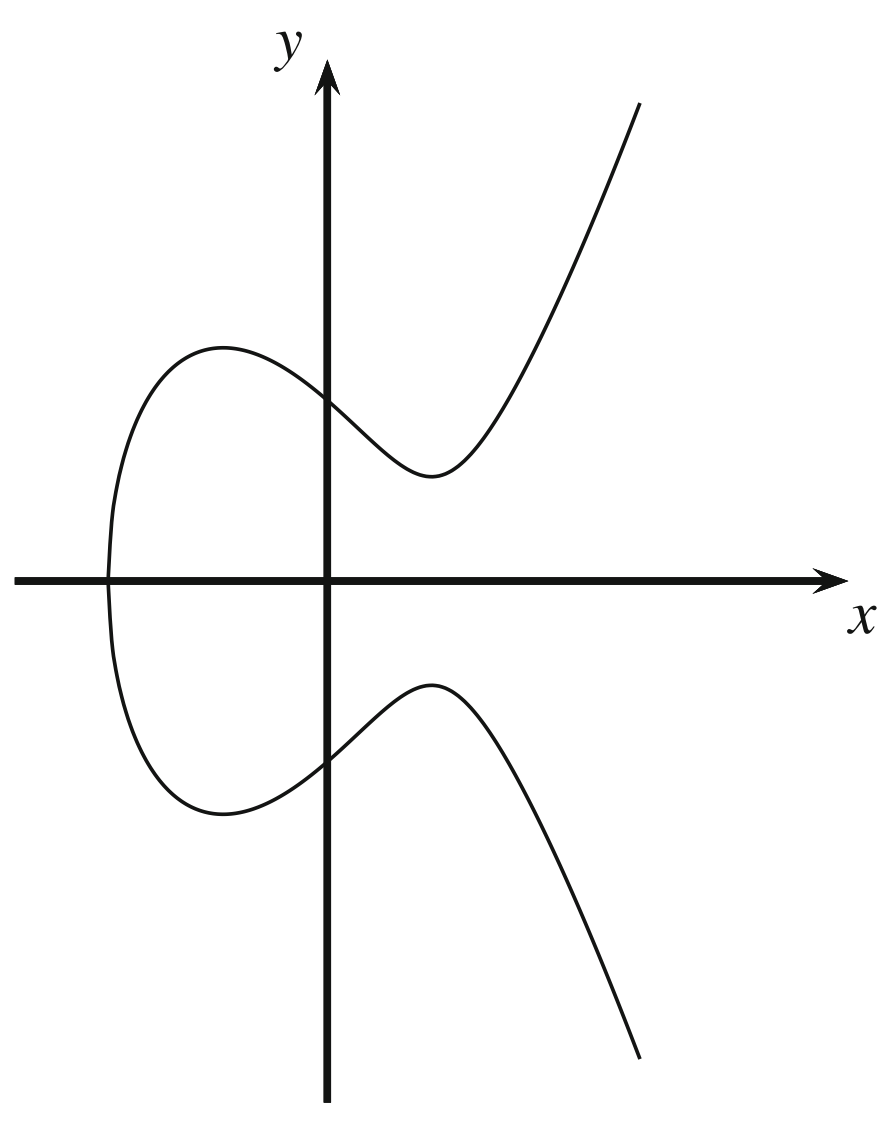
\includegraphics[width=0.3\textwidth]{grafiken/Elliptische_Kurve.PNG}
    \caption[r]{r}
    \label{fig:XXXX}
\end{figure}
Damit elliptische Kurven sinnvoll in der Kryptologie eingesetzt werden können, muss die Polynomgleichung über einem Primkörper betrachtet werden. Das heißt einfach gesprochen, alle Berechnungen werden modulo $p$ durchgeführt.
\paragraph{Definition: Elliptische Kurven über Primkörpern}
Die \textit{elliptische Kurve} über $\mathbb{F_p}$, ist die Menge aller Punkte $(x,y)$ mit $x,y \in \mathbb{F_p}$, welche die folgende Gleichung erfüllen: 
\begin{center}
$y^2 \equiv x^3 + ax + b$ mod $p$, wobei $a,b \in \mathbb{F_p}$
\end{center} 
und die Bedingung  $$4a^3 + 27b^3 \neq 0$$ gelten müssen. Zu der elliptischen Kurve gehört des Weiteren auch der imaginäre \textit{Punkt im Unendlichen} $\mathcal{O}$.\\

Durch die Bedingung XY werden sog. Singularitäten ausgeschlossen. Andernfalls gäbe es Punkte, deren Tangente nicht wohldefiniert ist, was für das Rechnen auf elliptischen Kurven jedoch erforderlich ist.

Nachdem elliptische Kurven nun definiert wurden, stellt sich die Frage, wie diese in der Kryptographie eingesetzt werden können. Wenn wir uns an das in Kapitel XY zurückerinnern, wird für die Konstruktion eines \textbf{DLP}s eine zyklische Gruppe benötigt. Eine eben solche findet sich in der Punktmenge der elliptischen Kurve wieder. Offen bleibt wie die Gruppenoperation definiert ist. Diese muss die in Kapitel XY geforderten Gruppengesetze erfüllen.\\

Als Symbol für die Gruppenoperation wird das Additionszeichen $+$ verwendet. Durch die Gruppenoperation muss aus zwei Punkten $P = (x_1, y_2)$ und $Q= (x_2, y_2)$ der Kurve ein dritter Punkt $R$ auf der Kurve berechnet werden. 
$$P + Q = R$$ $$(x_1, y_1) +  (x_2, y_2) = (x_3, y_3)$$
Am verständlichsten lässt sich diese Operation grafisch zeigen.

Elliptische Kurven über endlichen Körpern können grafisch nicht sinnvoll dargestellt werden. Ihre Form und Arithmetik lassen sich jedoch gut veranschaulichen wenn man sie auf $\mathbb{R}$ abbildet. Im Folgenden betrachten wir eine Elliptische Kurve, dargestellt in einem kartesischen Koordinatensystem, um die Gruppeneigenschaften bezüglich der Punktaddition zu zeigen. Hierbei sind nun zwei Fälle zu unterscheiden.\\

\textbf{Punktaddition $P + Q$:}
Falls $P \neq Q$ erfolgt die geometrische Konstruktion, indem zunächst eine Grade durch die beiden Punkte gelegt wird. Aufgrund der Kurveneigenschaften hat diese immer einen dritten Schnittpunkt mit der Kurve. Dieser wird an der $x$-Achse gespiegelt um den gesuchten Punkt $R$ zu erhalten. Abbildung XY zeigt die beschriebene Konstruktion.

\begin{figure}[H]
    \centering
    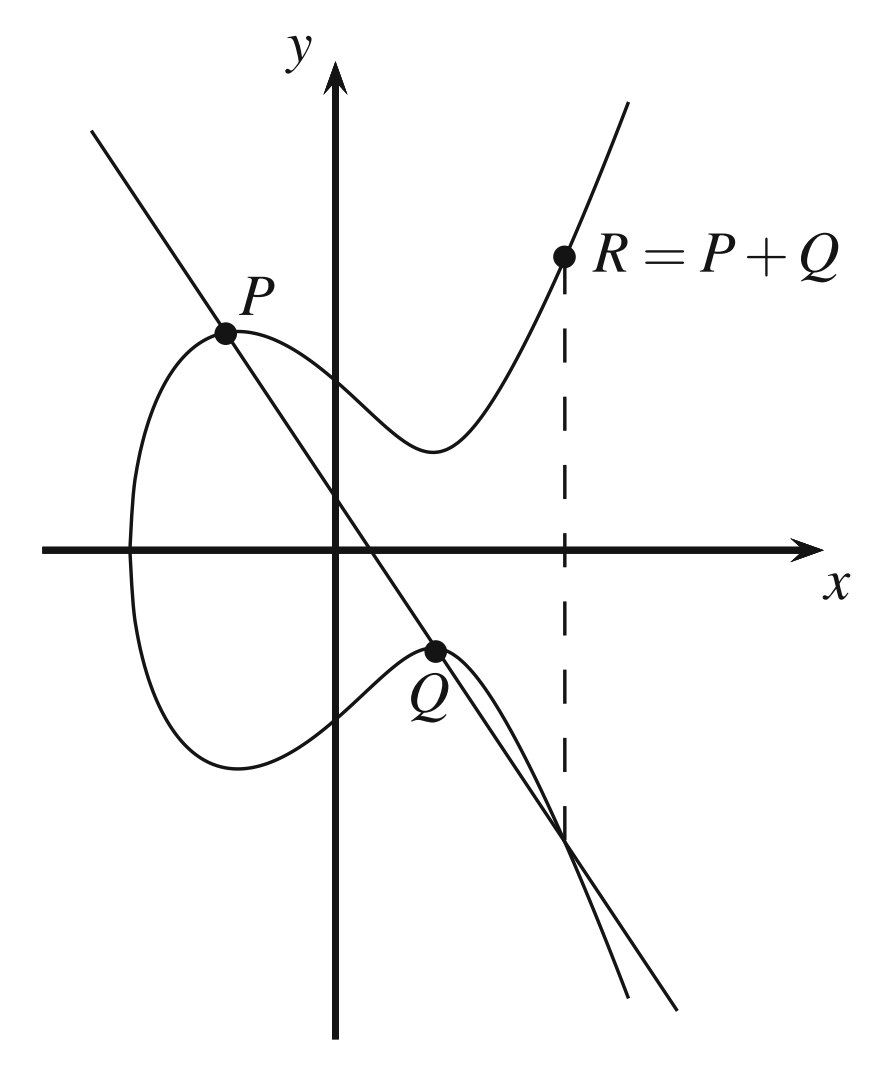
\includegraphics[width=0.3\textwidth]{grafiken/Punktaddition.PNG}
    \caption[Punktaddition]{r}
    \label{fig:Punktaddition}
\end{figure}

\textbf{Punktverdopplung $P + P$:}
Falls P und Q identisch sind erfolgt die geometrische Konstruktion, indem eine Tangente an den Punkt $P$ angelegt wird. Diese liefert wieder einen weiteren Schnittpunkt mit der Kurve, welcher an der $x$-Achse gespiegelt wird um den Punkt $R$ zu erhalten. Anstatt $R = P + Q$ schreibt man in diesem Fall $R = P + P = 2P$   Abbildung XY zeigt die beschriebene Konstruktion. 

\begin{figure}[H]
    \centering
    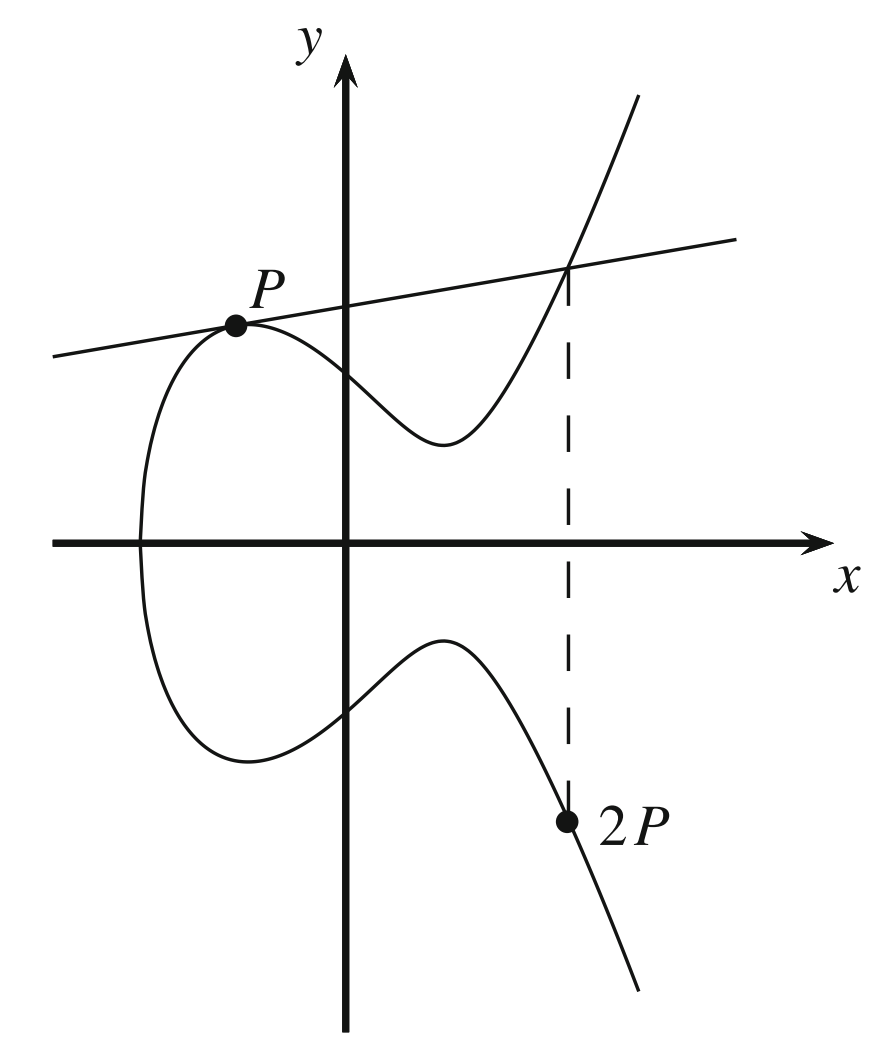
\includegraphics[width=0.3\textwidth]{grafiken/Punktverdopplung.PNG}
    \caption[Punktverdopplung]{r}
    \label{fig:Punktverdopplung}
\end{figure}

Nach dieser grafischen Veranschaulichung sollte es leichter fallen die folgenden Formeln für die Punktaddition bzw. Punktverdopplung nachvollziehen zu können. Die Gruppenoperation existiert in jedem Körper, weshalb die Berechnung von $R$, wie grade gezeigt über den reellen Zahlen $\mathbb{R}$, als auch über einem Primkörper $\mathbb{F}_p$ durchgeführt werden kann.\\

Die Formeln für die Punktaddition und - verdopplung auf elliptischen Kurven können anhand der grade gezeigten Veranschaulichung hergeleitet werden. Das Vorgehen hierbei ist prinzipiell recht simpel.\\ 

Gegeben ist die Gleichung der elliptischen Kurve $y^2 = x^3 +ax + b$ und die Punkte $P = (x_1, y_1)$ und $Q = (x_2, y_2)$. Zunächst ist die Geradengleichung der Sekante durch $P$ und $Q$ zu ermitteln. Eine Grade im Allgemeinen hat die Form $$g: y = sx + m.$$ Der Parameter $s$ ist dabei die Steigung der Geraden und $m$ ist der Schnittpunkt mit der $y$-Achse. Die Steigung $s$ lässt sich wie gewohnt durch Anlegen des Steigungsdreiecks berechnen, also mit der Formel $$s = \frac{y_2 - y_1}{x_2  - x_1}.$$

Zur Bestimmung des Schnittpunkts mit der $y$-Achse kann nun einer der beiden Punkte $P$ oder $Q$ in die Geradengleichung $y = \frac{y_2 - y_1}{x_2  - x_1} * x + m$ eingesetzt werden. Wenn wir $P = (x_1, y_1)$ einsetzen erhalten wir die folgende Gleichung $$y_1 = \frac{y_2 - y_1}{x_2  - x_1} * x_1 + m\text{,}$$ welche nach $m$ aufgelöst folgendermaßen aussieht: $$m = y_1 - \frac{y_2 - y_1}{x_2  - x_1} * x_1$$
Durch Einsetzten aller Parameter in die obige Geradengleichung ergibt sich $$y = \frac{y_2 - y_1}{x_2  - x_1} * x + y_1 - \frac{y_2 - y_1}{x_2  - x_1} * x_1$$ für die gesuchte Gerade $g$ durch die Punkte $P$ und $Q$. Um den dritten Schnittpunkt dieser Geraden $g$ mit der elliptischen Kurve $E$ zu ermitteln, sind beide Kurven gleichzusetzen. Da es für das weitere Vorgehen keine Rolle spielt und es der Übersichtlichkeit dient, werden im Folgenden wieder die Parameter $s$ und $m$ statt eben gezeigten Konkretisierungen verwendet. Es ergibt sich die Gleichung $$(sx+m)^2 = x^3 + ax + b\text{.}$$ Nach ausmultiplizieren erhalten wir $$0 =  x^3 - s^2x^2 + (a-2sm)\cdot x - m^2+b$$

Im Normalfall ist das allgemeine Lösen eines solchen kubischen Polynoms nicht trivial. Wir haben hier jedoch den Vorteil, dass zwei der drei Schnittpunkte von $g$ mit $E$ schon bekannt sind. Fassen wir das Polynom als Funktion $$f(x) = x^3 - s^2x^2 + (a-2sm)\cdot x - m^2+b$$ auf, so sind wir Im Grunde auf der Suche nach den Nullstellen dieser kubischen Funktion. Da die Punkte $P$ und $Q$ auf der Geraden g sowie auf der elliptischen Kurve E liegen, lösen sie die obige F
Gleichung, sind also Nullstellen der Funktion $f(x)$. Daraus folgt, dass die Funktion $f(x)$ restlos durch $(x-x_1)$ und $(x-x_2)$ geteilt werden kann um den Funktionsgrad zu verringern.
$$f(x) \div (x-x_1) \cdot (x-x_2) = l(x) \text{  Rest }0$$
Da $f(x)$ den Grad 3 hat, muss $l(x)$ den Grad 1 haben und durch $l(x) = ux + v$ beschrieben werden können. Da $$l(x) + (x-x_1) \cdot (x-x_2) = g(x)\text{,}$$ muss auch gelten $$u \cdot x \cdot x \cdot x  = x^3\text{,}$$ weshalb $u = 1$ gelten muss. Daraus ergibt sich $$l(x) = x + v \text{.}$$ Somit ist $x_3 = -v$ eine weitere Nullstelle von $f(x)$. Es folgt also $$g(x) = (x-x_1) \cdot (x-x_2) \cdot (x-x_3)$$, woraus durch ausmultiplizieren $$f(x) = x^3 - (x_1 + x_2 + x_3) \cdot x^2 + (x_1 x_2 + x_1 x_3 + x_2 x_3) * x - x_1 x_2 x_3$$ entsteht. Vergleicht man nun diese Darstellung mit der obigen also $$f(x) = x^3 - s^2x^2 + (a-2sm)\cdot x - m^2+b$$, so folgt durch Koeffizientenvergleich $$s^2 = x_1 + x_2 +x_3$$ also $$x_3 = x^2 -x_1 - x_2$$

Um die Formel für $y_3$ zu ermitteln kann nun der Punkt $R$ in die Formel für $s$ eingesetzt werden. Dies ist möglich, da der Punkt $R$ auf der Gleichen geraden wie $P$ und $Q$ liegt, weshalb aus die Steigung $s$ identisch ist.
Es gilt also $$s = \frac{y_2 - y_1}{x_2  - x_1} = \frac{y_3 - y_1}{x_3  - x_1}.$$ 
Aufgelöst nach $y_3$ ergibt sich also $$y_3 = s \cdot (x_3 - x_1) + y_1 \text{.}$$
Da der Schnittpunkt an der $x$-Achse gespiegelt wird um $R$ zu erhalten müssen die Vorzeichen in der Formel für $y$ noch gedreht werden. Final ergeben sich also die Formeln:
$$x_3 = s^2 + x_1 - x_2$$
$$y_3 = s \cdot (x_1 - x_3) y_1$$






\textbf{Formel: Punktaddition und -verdopplung auf elliptischen Kurven:}
$$x_3 = s^2 - x_1 - x_2$$
$$y_3 = s(x_1 - x_3) - y_1$$,
wobei

$$s = \begin{cases}
	\frac{y_2 - y_1}{x_2 -x_1} & \text{, falls } P \neq Q \text{ (Punktaddition)}\\
	\frac{3x_1^2 + a}{2y_1} & \text{, falls } P = Q \text{ (Punktverdopplung)}
	\end{cases}
$$

Zur Erfüllung der Gruppeneigenschaften wird außerdem ein neutrales Element $\mathcal{O}$ benötigt. Alle Punkte $P$ der elliptischen Kurve müssen die Eigenschaft $P + \mathcal{O} = P$. Da kein Punkt der elliptischen Kurve diese Eigenschaft erfüllen kann, wird der imaginäre \textit{unendlich ferne Punkt} als neutrales Element $\mathcal{O}$ definiert. Dieser Punkt liefert den dritten \textit{Schnittpunkt} mit der Kurve im Falle, dass ein Punkt $P$ und der bezüglich der $x$-Achse gegenüberliegende Punkt $-P$ addiert werden. Abbildung XY zeigt den Fall grafisch.

Die Existenz eines neutralen Elements ermöglicht die Definition eines Inversen $-P$ für jeden Punkt $P$ auf der Kurve, für welches $P + (-P) = \mathcal{O}$. Wie Abbildung XY  entnommen werden kann, ist für den Punkt $P = (x_p, y_p)$ das Inverse also $-P = (y_p, -y_p)$ zu definieren. In einem Primkörper berechnet sich die negative $y$-Koordinate durch $-y_p = p - y_p$.
 
\section{Punktbestimmung}
Die Arithmetik für Elliptische Kurven wurde bereits besprochen. Nun wird erarbeitet, wie man die Punkte einer elliptischen Kurve bestimmt. Doch was ist ein Punkt einer elliptischen Kurve? Im Foglenden wird erklärt, was ein Punkt auf einer elliptischen Kurve ist und wie diese berehcnet werden können. Die Erklärungen werden anschließend anhand einiger Beispiele näher erläutert. Anschließend wird Python-Code präsentiert, welcher die Punktbestimmung für eine elliptische Kurve mit p > 3 durchführt und die Punkte anschließend in der Konsole ausgibt.

\subsection{Rechnerische Grundlagen}
Viele Mathematiker suchten eine Formel, mit denen sich die Anzahl der Punkte einer elliptischen Kurve schätzen lässt, ohne dass man diese vorher aus- oder berechnen muss. Joseph H. Silverman beweist in seinem Buch einen mathematischen Satz aus der Zahlentheorie, welcher eine allgemeine Aussage über die Anzahl der rationalen Punkte auf einer elliptischen Kurve trifft \cite[vgl.][S. 138]{silverman}. Dieser Satz kann also herangezogen werden, um eine ungefähre Abschätzung über die Anzahl der Punkte auf einer elliptischen Kurve über einem Primkörper p zu treffen. Bei dem mathematischen Satz handelt es sich um die Hasse–Weil–Schranke. Diese wird im allgemeinen dafür benutzt, um die Anzahl der Lösungen der Gleichung und der Bedingungen aber auch für die Einschränkung des Lösungsraums. Die Hasse-Weil-Schranke wird angelehnt an \cite[vgl.][S. 181]{reinholdhuebl} wie folgt beschrieben. Sei k = $\mathbb{F}_p$ ein endlicher Körper und $\overline{E}$ eine elliptische Kurve über k, dann gilt
\begin{center}
$p + 1 - 2 * \sqrt{p} \leq | \overline{E} | \leq p + 1 + 2 * \sqrt{p}$
\end{center} 

Was ist jedoch die Hauptaussage der Hasse-Weil-Schranke? Sie besagt, dass sich bei großen p die Anzahl der Elemente der elliptischen Kurve in der Größenoprdnung von p bewegen. Diese Schranke bildet hierbei eine obere und untere Grenze. Die Anzahl der Punkte bewegt sich also innerhalb dieser Schranke. Dies ist für elliptische Kurven mit kleinem p uninteressant, jedoch wird diese Schranke für elliptische Kurven mit großem gewählten p, was in der Kryptographie gängig ist, relevant.\\


Doch wie lassen sich die Punkte konkret berechnen? Um diese Frage zu beantworten, müssen wir noch einmal die Grundlagen für elliptische Kurven aufgreifen. Wie Reinhold Hübl in seinem Manuskript der Kryptologie \cite[vgl.][S. 157]{reinholdhuebl} erläutert, ist eine elliptische Kurve mit den Charakteristiken char(k) = 0 oder char(k) = 3 eine Kurve, die durch ein Polynom der Form
\begin{center}
$F(X, Y) = Y^{2} - X^{3} - aX - b$
\end{center} 

mit $a, b \in k$ dargestellt ist, für die $4a^3 + 27b^2 \neq 0$  $\in k$ gilt.\\

Stellt man die Gleichung der Funktion nach $y^{2}$ um, dann erhält man folgende Gleichung in zwei Variablen:
\begin{center}
$y^{2} =  x^{3}$ + ax + b  mod(p),
\end{center}

wobei $a, b \in \mathbb{F}_p$. Diese Gleichung ist der Schlüssel für die im Voraus aufgeworfene Frage, was ein Punkt einer elliptischen Kurve ist. Diese sind nämlich alle Punkte (x, y), welche die Gleichung lösen.\\

Um die Punkte auf einer Kurve zu berechnen, prüft man zunächst, ob es sich bei der betrachteten Kurve um eine elliptische Kurve mit p > 3 handelt. Dafür arbeitet man mit der Formel  $4a^3 + 27b^2 \neq 0$. Man setzt die Parameter a und b der vermeintlichen elliptischen Kurve ein. Wenn die linke Seite $\neq 0$ ist, dann handelt es sich bei der besagten Kurve tatsächlich um eine elliptische Kurve mit p > 3. Rechnen wir dies nun einmal schematisch durch. Gegeben ist eine Funktion F mit
\begin{center}
$F(X, Y) = Y^{2} - X^{3} + 3X - 3 \in \mathbb{F}_{13}$
\end{center} 

Wie man der Funktion entnehmen kann ist a = - 3 = 10 und b = 3 in $\mathbb{F}_{13}$. Diese setzen wir nun in die Formel ein.
\begin{center}
$4 * 10^3 + 27 * 3^2 = 6 \neq 0$ mod(13)
\end{center} 

Da 6 $\neq$ 0 ist definiert die Funktion eine elliptische Kurve in $\mathbb{F}_{13}$. Die Abbildung \ref{fig:kurve_beispiel_1_punktberechnung} zeigt die Zeichnung der Funktion dieser elliptischen Kurve über den reellen Zahlen im kartesischen Koordinatensystem: 

\begin{figure}[H]
    \centering
    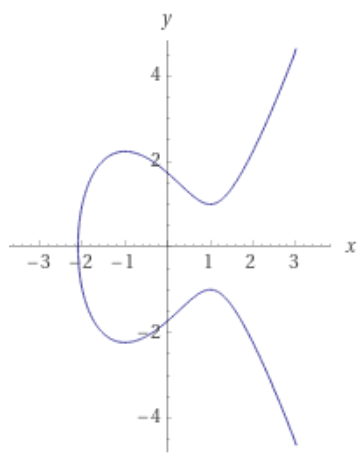
\includegraphics[width=0.5\textwidth]{grafiken/kurve_beispiel_1_punktberechnung.png}
    \caption[Zeichnung der elliptischen Kurve]{Zeichnung der elliptischen Kurve \\ Quelle: Wolframalpha}
    \label{fig:kurve_beispiel_1_punktberechnung}
\end{figure}

Nachdem man allgemein geprüft hat, ob es sich bei der besagten Funktion um eine elliptische Kurve handelt, geht es jetzt um die Findung der Lösungen der umgestellten Gleichung, um alle Punkte zu finden. Dafür gibt es mehrere Möglichkeiten. Die Möglichkeiten haben unterschiedliche Zeit- und Rechenkomplexitäten, wodurch sich die Lösungsmöglichkeiten differenzieren lassen. Je nach Anwendungsfall lohnt sich die Implementierung einer anderen Lösung. Im Folgenden sind drei Möglichkeiten zur Berechnung aller Punkte auf elliptischen Kurven aufgezählt:

\begin{itemize}
\item Brute-Force
\item Punktaddition und Punktverdopplung
\item Algorithmischer Brute-Force
\end{itemize}

Neben dieser drei gängigen Methoden werden in der Mathematik und in der Kryptografie auch die Barrett-Reduktion und weiterhin auch eine Methode, bei welcher sich die Symmetrie zur x-Achse der elliptischen Kurve zur Berechnung zunutze gemacht wird, genutzt. Um diese soll es jedoch nicht gehen. In den folgenden zwei Unterkapiteln wird die Berechnung der Punkte über Brute-Force mit zwei Methoden sowie über die Punktaddition und -verdopplung erläutert und mittels Beispielen verständlich erklärt.

\subsection{Punktberechnung: Brute-Force-Methode}
Wie bereits erläutert wurde, ist die umgestellte Gleichung der elliptischen Kurve in zwei Variablen folgende:
\begin{center}
$y^{2} =  x^{3}$ + ax + b  $\in \mathbb{F}_{p}$
\end{center}

Da die linke Seite mit $y^{2}$ offensichtlich quadratisch ist, muss am Ende auf beiden Seiten der Gleichung die Quadratwurzel gezogen werden, um die Gleichung zu lösen und im weiteren Sinne Punkte auf der Kurve zu finden. Da dies umständlich und im endlichen Körper $\mathbb{F}_{p}$ schwer zu realisieren ist, wird die rechte Seite bis zu einem Quadrat aufgelöst. Dafür muss man als erstes bestimmen, welche Werte in der entsprechenden Restklasse der elliptischen Kurve Quadrate sind. Die Quadratprüfung ist dabei simpel: Man geht jedes Element in $\mathbb{F}_{p}$ von 0 bis p-1 durch und prüft, ob das quadrierte Element in der Restklasse ein Quadrat ist. Hierbei geht es um keine komplexe Rechnung, sondern lediglich um stupides ausprobieren. Zur Verdeutlichung folgendes Beispiel: Wir haben den Körper $\mathbb{F}_{5}$. Der Körper beinhaltet die Elemente $\mathbb{F}_{5}$ = {0, 1, 2, 3, 4}. Die Quadrate mitsamt ihrer Wurzeln sind folgende:
\begin{center}
$0 = 0^{2} \qquad 1 = 1^{2} = 4^{2} \qquad 4 = 2^{2} = 3^{2}$
\end{center}

Die Zahlen 0, 1 und 4 sind demnach in $\mathbb{F}_{5}$ Quadrate. Die Wurzeln wurden der Vollständigkeit halber ebenfalls obig rechts des Quadrates notiert. Man berechnet die Quadrate nach folgendem Schema:

\begin{enumerate}
\item Man hat k mit k $\in \mathbb{F}_{p}$
\item Man beginnt bei k = 0
\item Es wird quadriert mit $k^{2}$
\item Der Wert von $k^{2}$ in $\mathbb{F}_{p}$ wird ermittelt, dafür rechnet man $k^{2}$ mod(p)
\item Die ermittelte Zahl ist ein Quadrat in $\mathbb{F}_{p}$
\item Man wiederholt alle Schritte mit allen k von 0 bis p-1
\item Am Ende hat man alle Quadrate und ihre zugehörigen Wurzeln
\end{enumerate}

Dies wird anhand eines ausführlichen Beispiels deutlich. Sei p = 11 und somit $\mathbb{F}_{p}$ = $\mathbb{F}_{11}$. 

\begin{itemize}
\item $0^{2} \equiv 0 $  mod(11)
\item $1^{2} \equiv 1 $  mod(11)
\item $2^{2} \equiv 4 $  mod(11)
\item $3^{2} \equiv 9 $  mod(11)
\item $4^{2} \equiv 5 $  mod(11)
\item $5^{2} \equiv 3 $  mod(11)
\item $6^{2} \equiv 3 $  mod(11)
\item $7^{2} \equiv 5 $  mod(11)
\item $8^{2} \equiv 9 $  mod(11)
\item $9^{2} \equiv 4 $  mod(11)
\item $10^{2} \equiv 1 $  mod(11)
\end{itemize}

Wenn man die Null dazuzählt, hat $\mathbb{F}_{11}$ die Quadrate 0, 1, 3, 4, 5, 9. Im Folgenden sind die Quadrate mitsamt ihrer Wurzeln aufgeschrieben:

\begin{itemize}
\item Quadrat: 0 $\quad$ Wurzel 1: $0^{2}$
\item Quadrat: 1 $\quad$ Wurzel 1: $1^{2} \quad$ Wurzel 2: $10^{2}$
\item Quadrat: 3 $\quad$ Wurzel 1: $5^{2} \quad$ Wurzel 2: $6^{2}$
\item Quadrat: 4 $\quad$ Wurzel 1: $2^{2} \quad$ Wurzel 2: $9^{2}$
\item Quadrat: 5 $\quad$ Wurzel 1: $4^{2} \quad$ Wurzel 2: $7^{2}$
\item Quadrat: 9 $\quad$ Wurzel 1: $3^{2} \quad$ Wurzel 2: $8^{2}$
\end{itemize}

Die berechneten Quadrate und Wurzeln sind nötig, um die Punkte zu bestimmen. Um dies zu bewerkstelligen, wird die Gleichung der elliptischen Kurve in zwei Variablen benötigt. Um die benötigte Formel zu erhalten, überführen wir die Ausgangsgleichung in zwei Variablen in eine Funktionsgleichung mit einer Variablen:
\begin{center}
$y^{2} =  x^{3}$ + ax + b  $\in \mathbb{F}_{p} \qquad \Longrightarrow \qquad f(x) =  x^{3}$ + ax + b  $\in \mathbb{F}_{p}$
\end{center}

Diese Funktionsgleichung ist der Ausgangspunkt für die Berechnung der Punkte. Man setzt nun alle x-Werte von 0 bis p-1 in die Funktionsgleichung ein. Jene x-Werte, welche die Quadrate ergeben, werden für die Punktbestimmung benötigt. Nehme als Beispiel p = 11. Wir haben die Quadrate und die Wurzeln oben bereits ausgerechnet. Sei weiterhin die Gleichung einer elliptischen Kurve E gegeben mit
\begin{center}
$F(X, Y) =  Y^{2} - X^{3}$ - X - 3  $\in \mathbb{F}_{11}$
\end{center}

Damit ist die umgestellte Gleichung in zwei Variablen und die Funktionsgleichung mit einer Variablen
\begin{center}
$y^{2} =  x^{3}$ + x + 3 $\qquad \Longrightarrow \qquad f(x) =  x^{3}$ + x + 3 $\in \mathbb{F}_{11}$
\end{center}
Setzen wir nun alle Elemente von 0 bis p-1 in die FUnktionsgleichung ein und schauen uns die Ergebnisse an.

\begin{itemize}
\item $f(0) =  0^{3}$ + 0 + 3 = 3 $\in \mathbb{F}_{11} \qquad \Longrightarrow \qquad$ Quadrat
\item $f(1) =  1^{3}$ + 1 + 3 = 5 $\in \mathbb{F}_{11} \qquad \Longrightarrow \qquad$ Quadrat
\item $f(2) =  2^{3}$ + 2 + 3 = 2 $\in \mathbb{F}_{11}$
\item $f(3) =  3^{3}$ + 3 + 3 = 0 $\in \mathbb{F}_{11} \qquad \Longrightarrow \qquad$ Quadrat
\item $f(4) =  4^{3}$ + 4 + 3 = 5 $\in \mathbb{F}_{11} \qquad \Longrightarrow \qquad$ Quadrat
\item $f(5) =  5^{3}$ + 5 + 3 = 1 $\in \mathbb{F}_{11} \qquad \Longrightarrow \qquad$ Quadrat
\item $f(6) =  6^{3}$ + 6 + 3 = 5 $\in \mathbb{F}_{11} \qquad \Longrightarrow \qquad$ Quadrat
\item $f(7) =  7^{3}$ + 7 + 3 = 1 $\in \mathbb{F}_{11} \qquad \Longrightarrow \qquad$ Quadrat
\item $f(8) =  8^{3}$ + 8 + 3 = 6 $\in \mathbb{F}_{11}$
\item $f(9) =  9^{3}$ + 9 + 3 = 4 $\in \mathbb{F}_{11} \qquad \Longrightarrow \qquad$ Quadrat
\item $f(10) = 10^{3}$ + 10 + 3 = 1 $\in \mathbb{F}_{11} \qquad \Longrightarrow \qquad$ Quadrat
\end{itemize}

Die Ergebnisse zeigen dass die folgenden x-Werte Quadrate definieren: 0, 1, 3, 4, 5, 6, 7, 9, 10. Bis jetzt wurde der einfache Brute-Force durchgeführt. Man muss nur noch wenige Schritte durchführen, um die Punkte auf der elliptischen Kurve zu bestimmen. Wir haben jetzt die Quadrate, die dazugehörigen Wurzeln sowie die x-Werte, welche Quadrate sind. Wie kombiniert man diese, um die Punkte auf der elliptischen Kurve zu erhalten?

Konnte ein y-Wert zu einem x-Wert gefunden werden, dann ist (x, y) $\in$ E. Beide Werte zusammen ergeben einen Punkt P(x, y) auf der elliptischen Kurve. IST TRASH, WIRD ABER FÜR COPY PASTE BENÖTIGT

\subsection{Punktberechnung: Algorithmische Brute-Force-Methode}
U

\subsection{Punktberechnung: Punktaddition und -verdopplung}
U

\subsection{Implementierung in Python}
U




































